\chapter{Introduction}
\label{ch:introduction}
\pagenumbering{arabic}
\pagestyle{headings}

This project aims to simplify and enhance the management and monitoring capabilities of network's administrators using Bird Daemon software on top of an OpenWrt/LEDE-based Firmware. It is a second iteration in the development of an existing configuration integration package already being used by OpenWRT/LEDE's community. Section \ref{ch:backc} introduces the key concepts used in in the introduction and as part of the dissertation itself.

\section{Background Concepts}
\label{ch:backc}
The following subsections are intended to be self-contained definitions for contents recurrently referenced in this dissertation, sorting them by scope (from top to bottom). The two highest-level topics covered are OpenWrt and LEDE environments and project's target network.
\subsection{OpenWrt/LEDE Project}
\label{subsec:owrtlp}
OpenWrt, and its Fork LEDE (Linux Embedded Development Environment), are Open Source Linux-based firmwares primarily focused on commodity routers, but aiming to work in any Linux-based system. This firmware supports a wide variety of manufacturer's hardware and also a wide range of software, services and routing protocols to enhance, secure and efficiently operate as a standalone router and service provider. This community-driven firmware uses different internal GIT source repositories as well as the GitHub service, which is the most widely used. As any other open source project using GIT, it allows users to contribute to it by doing changes in their own repository forks and then creating Pull Requests in GitHub's website in order to get their changes approved and integrated in the official stream. This procedure is followed in all the different repositories that the project owns and has a big number of reviewers to protect the project's code quality and the system's stability.

\subsubsection{UCI}
The Unified Configuration Interface aims to centralise OpenWrt's packages and the system configuration. This mechanism is widely used for almost, if not all, the packages working in OpenWrt. UCI allows you to easily, and in a human-readable manner, simplify administration overheads. For reference, the following UCI configuration item configures the loopback interface: 

\begin{lstlisting}[language=bash,caption={Loopback network interface's configuration using UCI.}]
config interface 'loopback'
	option ifname 'lo'
	option proto 'static'
	option ipaddr '127.0.0.1'
	option netmask '255.0.0.0'
\end{lstlisting}

\subsubsection{LUCI}
Lua UCI is OpenWrt's implementation provide a graphical to manage UCI settings via web pages (UI is generated on Server side) following a Model-View-Controller software pattern implementation and using Lua programming language.

LUCI's main components are:
\begin{itemize}
    \item CBI (Model): CBI files include the UCI definition and \textit{describe} HTML's presentation (e.g optional/mandatory properties, order of apparition, and all the required logic to validate entered data through the forms).
    \item Controller: Web pages definition (e.g data, pages order or rendering target) and communication functions required by the Model (CBI) page.
    \item View: HTML templates defining how a page, section or specific element is represented.
\end{itemize}

\subsubsection{LUCI2}
\label{sub:sub:luci2}
LUCI2 is the 2\textsuperscript{nd} generation of OpenWrt's UCI UI modeling architecture. This second version uses client side page generation technologies (HTML, CSS and JavaScript) to enhance and simplify UI creation and also releasing router's resources from handling UI creation and management. Moreover, this new version uses a standard communication process between client's browser and router's backend http server: standard XMLHTTPRequest (XHR) API. This standard API uses HTTP Requests to transfer objects by embedding them in the URL but avoiding page reloads. This mechanism's most common object format is JavaScript Object Notation (JSON).

Because of the new requirements emerged as consequence of moving UI's creation from the server side to the client side, we need a mechanism together with an architecture supporting it (explained in section \ref{sub:luci2arch}), to query router's data:
\begin{itemize}
    \item Universal Bus (uBus) is a service that allows communication between different services. It is implemented to act as a pipe for packages or protocols to register their APIs in a shared \textit{namespace}. uBus provides its own httpd server plugin to communicate with client's browser using it.
\end{itemize} 

In order to use uBus capabilities, services must integrate it in their code. For those packages not being able (or not willing) to do it, uBus also provides an alternative registration method:
\begin{itemize}
    \item RPCd (Remote Procedure Calls Daemon) is an HTTP backend server implementation for client-server communication calls in network-based systems. In OpenWrt's case, queries are mainly sent from client's browser to the backend server (RPCd).
    
    This backend server allows non-uBus-integrated services to register an API with it, using Shell commands to define required functions. Services registering to RPCd will be able to query uBus through client calls but these APIs will need to handle request's data and data object's format.
\end{itemize}

Finally, this new version is still experimental. There is not many documentation of its API definition, how to use or integrate it in a new or existing package and, therefore, it is complex to get the full picture of how this architecture works or how to integrate it. 

\subsection{Bird Daemon}
Bird Daemon (from now onwards Bird)\cite{bird} is an open source Internet Routing service that allows network administrators to simplify route sharing configuration, management and monitoring of different routing protocols by using Routing tables as \textit{transferable} knowledge and a powerful filtering c-like language to achieve it with really fine-grained results. Bird manages its own configuration also following the same c-like scheme, which was the main goal of my 2014 project: to automate and simplify it by using UCI instead and letting the Package do the translation to Bird configuration.

Bird current version is 1.6.3 and its functionality is split in two different Daemons: one for IPv4 (Bird4) and one for IPv6 (Bird6). This version supports the following routing protocols:

\subsubsection{Routing Protocols}
\begin{itemize}
    \item Babel: IGP (\Gls{igp}) distance-vector protocol stated as being in alpha stage of adoption.
    This protocol is not available to automate through our Package yet.
    \item \textbf{Open Shortest Path First - OSPF}: IGP link-state protocol fully supported for both IPv4 OSPFv2 and IPv6 OSPFv3.
    This protocol has some functionality available for IPv4 in the Package but is not fully functional and there is no UI supporting it. OSPF support is one of the top priorities for future Package improvements.
    \item \textbf{Routing Information Protocol - RIP}: IGP distance-vector protocol fully supported. This protocol is completely deprecated by other distance-vector protocols as OSPF, which are less constrained by network's scale.
    This protocol is not available to automate through our Package and, because it is obsolete, there are not plans to implement it in short term.
    \item \textbf{Border Gateway Protocol - BGP}: EGP (\Gls{egp}) path-vector protocol fully supported. This is the most common protocol for backbone networks and the key protocol for this project.
    This protocol is available to automate through the Package but only the most common or relevant options have been implemented. BGP's support finalisation is one of the top priorities for future Package improvements. 
\end{itemize}.

\subsubsection{Bird Support \textit{Protocols}}
\label{sub:sub:supproto}
The following list of Bird utilities have been named protocols. However, these are not real routing protocols but a number of supportive implementations of different functionalities or standard services to enhance and simplify Bird's management. This naming convention unifies Bird's implementation and configuration management, but it must not be mistaken for a real protocol.

\begin{itemize}
    \item \textbf{Static Protocol}: Bird's mechanism to implement \textit{smart} static routes. It allows  origin or pattern discrimination and modification. For example, to configure any route in 10.0.0.0/16 to be unreachable or to extend it with an attribute: \texttt{ospf\_metric = 100}.
    Static Protocol is available to automate through the Package.
    \item \textbf{Pipe Protocol}: Routing Tables are the main, and OS standard, knowledge units for Bird (e.g BGP \& OSPF primary tables). Pipe Protocol allows to connect different Routing Tables and to apply discrimination to the routes they share (e.g \texttt{BGP->OSPF accept all} and \texttt{OSPF->BGP accept} filtered to: \texttt{if net \~{} 10.0.0.0/8}).
    Pipe Protocol is available to automate through the Package.
    \item \textbf{Direct Protocol}: Route generator for any targeted interface. Bird uses pattern matching to include/exclude any network interface that we want to be encapsulated as a single bunch of \textit{device} routes.
    Direct Protocol is available to automate through the Package.
    \item \textbf{Device Protocol}: This functionality is required in most of the Bird configurations and its main purpose is to gather key data from system's network interfaces in order to facilitate Bird's operation.
    Device Protocol is available to automate through the Package.
    \item \textbf{Kernel Protocol}: Bird's implementation to allow sharing routes between the Operative System Kernel Routing Tables and the ones designated by Bird.
    Kernel Protocol is available to automate through the Package. There are plans to improve this protocol as there is one process left to be automated through UI and it is top priority.
    \item \textbf{RAdv Protocol}: Implementation of the Router Advertisement Protocol (IPV6's Neighbour Discovery) allowing a fine-grained control of how often the neighbour discovery information is sent and which information is shared on them per target.
    RAdv Protocol is not available to automate through the Package. There are no plans to implement it in the short term. 
    \item \textbf{Biderectional Forwarding Detection - BFD Protocol}: This utility is a standalone tool for neighbours monitoring in order to foresee some protocol service disruptions by monitoring peers in a more efficient way than most protocols do. This protocol consists in a session created by real routing protocols (e.g OSPF and BGP) and its sole role is to notify them in case of an event. This protocol is almost fully supported (except of verbose mode and authentication).
    BFD Protocol is not available to automate through the Package. There are not plans to implement it in short the term.
\end{itemize}

\subsubsection{Bird Filter and Functions}
\label{sub:sub:filfun}
One of Bird's key functionalities is network routes filtering through scripting. Bird main configuration allows an administrator to define rules that routes imported or exported will need to be compliant with to avoid pass discrimination using its own programming simple \textit{language} (loops are not implemented). This language provides:
\begin{itemize}
    \item Functions: self-contained functionality required in several places. Their function is to reduce code's repetition but not to accept or drop routes.
    \item Filters: instructions executed by Bird on each route received (or about to be sent) through the different protocols in order to modify route's properties and to, according to the defined requirements, let the route pass or not.     
\end{itemize} 

\subsection{OpenWrt/LEDE's configuration integration package}
Bird-OpenWrt Package (from now onwards the Package) is an open source OpenWrt/LEDE-specific solution compound by four separated packages for UCI and LUCI configuration management and presentation for both IPv4 (bird4-uci and luci-app-bird4) and IPv6 (bird6-uci and luci-app-bird6) Bird implementations.

These packages provide administrators using Bird an user-friendly configuration scheme (UCI), automated configuration processes and graphical interface capabilities (LUCI) instead of its c-like configuration scheme. Specific implementation details are covered in chapter \ref{ch:implementation}.

This Package is currently part of OpenWrt's official stream (version 0.2) in GitHub and developers can contribute to it in the same way as with any other OpenWrt/LEDE component or service.

\subsection{Guifi.net}
\label{subsec:gn}
Guifi.net is a community-driven network working for and by its own users providing an affordable alternative for anyone willing to connect to the Internet. This network's principles are freedom; open design, administration and management; and neutrality. It was born in Catalonia as a wireless network (Access Point to Endpoint and Access Point to Access Point) but it has spread all over the world with about 33.124 active nodes (as 26/05/17) using roof antennas and, more recently, optical fiber deployments. This has made auspicious for other network topologies as mesh networks, making of Guifi.net a rich and heterogeneous network.

This network has its own Government Foundation, La Fundació Guifi.net, which main goals are to promote and protect network's principles defined in an operational and behavioural common regulation named \Gls{xoln}, support any company that adheres to XOLN's principles allowing them to be able to professionally operate and advertise themselves as Guifi.net service providers and, last but not least, to represent Guifi.net network and the internal service providers as a member (peer) of Catalan's Internet Exchange Point (CATNIX) bringing the possibility for any internal service provider to peer with other members to exchange traffic and routes\footnote{For reference, one of the latest incorporations as a member to CATNIX is AKAMAI service provider, thus making feasible for Guifi.net internal service providers to peer with this worldwide Content Delivery Network.}.

Finally, although Guifi.net main routing protocol is BGP for infrastructure and OSPF for internal routing, there are several isles operating as Mesh Networks using BMX6 dynamic routing protocol.


\subsection{Infrastructure vs Mesh Network Routing Protocols}
\label{subsec:dsrp}
Routing protocols' job is to receive a route and, according to its attributes and the information stored in the system, to redirect this route to the next step towards its destination or to drop it. However, each protocol follows different principles in order to achieve the best performance using different algorithms or paradigms. Moreover, depending on who is consuming the network and which are its requirements, we could prioritise either scalability, stability or resilience and prioritise how much critical are the previous characteristics for our consumers:

\begin{itemize}
    \item \textbf{Infrastructure Protocols}: commonly used in \textit{backbone} networks, which are commonly deployed in robust and powerful devices following a specific architecture. These protocols' strength is to be stable, robust and highly scalable. However, their main handicap is that it suffers from big overheads on topology changes. This means that these protocols are low/non fault tolerant and this is translated into longer convergence times (seconds to few minutes) in large-scale networks.

    \item \textbf{Mesh Protocols}: oppositely to backbone networks, mesh networks' strength is to be able to converge almost instantly after any topology event. These networks work in a cooperative manner in order to achieve a fully connected network (point-to-multipoint) where all the nodes share network's knowledge in order to optimise routes and nodes floods the network in order to keep network's topology knowledge up to date. This is a strong requirement due to the heterogeneity of these networks and that, some of them, are configured in unpredictable environments with high feasibility of suffering from topology changes. Nevertheless, this network's topology is built on the premise of being able to interconnect as many nodes as possible to each other to be able to quickly redirect network's transit to reach any node in the system, even on a topology change event.
\end{itemize}

\subsubsection{BGP}
\label{subsubsec:bgp}
BGP is a dynamic infrastructure IP routing protocol designed for large-scale internet topologies Autonomouos Systems routing entities (Autonomous Systems are internally compound by from small to mid scale networks acting as a single entity). Its routing algorithm relies on the best path according to route's attributes.

\subsubsection{BMX6}
\label{subsec:bmx6}
Batman-eXperimental6 \cite{bmx6} is a BATMAN (Better Approach To Mobile Adhoc Networking) mesh protocol's fork using different routing algorithms. This routing protocol is compatible with most of linux-like systems, it is optimised for IPv6 networks while it is also able to announce and receive IPv4 prefixes. This routing protocol uses a table-driven distance-vector approach (BMX6 tries to compose a routing table with all the source-destination entries and routes traffic according to the best path to reach the destination.

%%%%%%%%%%%%%%%%%%%%%%%%%%%%%%%%%%%%%%%%%%%%%
%%%%%%%%%%%%%%%%%%%%%%%%%%%%%%%%%%%%%%%%%%%%%
%%%%%%%%%%%%%%%%%%%%%%%%%%%%%%%%%%%%%%%%%%%%%

\section{Motivation}
\label{sec:motivation}
Back in 2014, while I was working on my BSc. dissertation at Universitat Politècnica de Catalunya, the department and, specifically, the investigation team I was working with, gave me the opportunity to participate in a \Gls{gsoc} project under the umbrella of Freifunk, to design, develop and demonstrate a package that would help to simplify the configuration of Bird as a software able to share routes between BMX6 mesh and BGP infrastructure networks. This solution was meant to be installed in \textit{border} nodes deployed in the Catalan community network Guifi.net and, therefore, production ready.

That project was successful and the result was an integration package using OpenWrt's well-known UCI/LUCI configuration mechanism to set up Bird through an user-friendly Web UI even without knowledge of Bird's syntax. However, GSoC's time frame was not enough to polish the package and to add other non-critical routing protocols. Moreover, the Package stopped being maintained later that year. Nevertheless, this OSS project has been on my \textit{backlog} of things I want to keep improving and also I have been queried some times by Víctor Oncins as this package is really helpful for network administrators but it is not mature enough for complex production environments available in Guifi.net.

Therefore, I have been really fortunate to have the opportunity to retake the development of this package as my MSc. project  and work together with Víctor as this has meant that I have had direct feedback from administrators using the tool in production environments and to improve its most critical features. Moreover, Víctor has also published a report on GitHub \cite{bgpbmx6} describing the main challenges found using the old version of the Package and a deep description of the environment.

\subsection{Bird Daemon administration issues}
\label{subsec:bdai}
As part of the GSoC project, the solution provided was not mature enough to fulfil all the requirements:
\begin{itemize}
    \item Tight time-frame forcing to prioritise the key capabilities to implement.
    \item Some key protocols were not enabled in the final solution because they were not relevant for GSoC's scope (e.g Pipe or Direct).
    \item Some routing protocols were not enabled in the final solution because they were not relevant for GSoC's scope (e.g OSPF or Babel).
    \item Some basic processes require manual (terminal) changes.
    \item No possible way to edit Filters or Functions files through Web UI.
    \item No Bird Daemon Status feedback (e.g no way to know if bird is running or failed to start through Web UI).
    \item No possible way to see Bird Daemon's Log information through Web UI.
    \item Bird's API changed (from Bird 1.4.3 to 1.6.3) making bird crash using base Package configuration.
    \item No possible way of monitoring Bird's current status (e.g full information for BGP connections).
\end{itemize}


\section{Scope of the project}
\label{sec:sotp}
This project's scope is to adopt some of the mentioned enhancements that are in consonance with command line based processes automation, to improve current UI's user experience and to align the Package with the current Bird Daemon's API in a 3 months time frame.

As a result of a \textit{backlog} prioritization, the following items were agreed (shown in priority order):
\begin{itemize}
    \item Update the Package to the latest Bird API.
    \item Update old version's disruptive issues (e.g disabled critical Protocols).
    \item Add Status, Log, Functions and Filters Bird capabilities graphical integration.
    \item Do a theoretical viability investigation of OpenWrt's uBus integration in order to gather Bird's live data and to be able to use it in the Package.
\end{itemize}


\subsection{Deviations from the original plan and future work}
While agreeing the original scope of the project, few extra ideas and tasks were planned but, as a matter of priorities and time constraints, some were dismissed or set as future work.

\begin{itemize}
    \item Add missing routing protocols: adopt OSPF routing protocol, other less critical routing protocols and functionalities, hence increasing the range of capabilities that are automated for administrators tu use  with no command line expertise required.
    \item Integrate next generation of Web UI using LUCI2: JavaScript-powered UI using uBus architecture instead of current LUA-based one.
    \item Implementation of uBus integration according to the results of the investigation done in this project.
    \item Comparative set of tests between Quagga and Bird Daemon solutions.
\end{itemize}

Most of these extra tasks are already documented as part of the Package Documentation Repository \cite{docng} and open for discussion if new requirements arise.

\subsubsection{Bird Daemon Vs. Quagga deployments}
There is a special reasoning behind not doing a comparative analysis of these two solutions. Of course the timing constrains have strongly influenced the decision of dropping this comparison from this project's scope, but there is also the big amount of evidence already collected for my GSoC2014 project, plus some new evidence found either in some reputable sources along with from Bird's own OSS Community proving that Bird Daemon has been far more stable, less resource eater and flexible (thanks to its Filter\&Function scripting language) than other well-known enterprise level solutions. This evidence and where it is coming from is available in Appendix \ref{app:ch:blinks}.


\section{Methodology and communication}
This project starts with the premise that there is no need for a wide initial investigation phase as the Package used was designed and developed by myself. Nevertheless, there are three foreseen introductory tasks:
\begin{itemize}
    \item Refresh the Package to the latest Bird Daemon version API. 
    \item Investigate, understand and document the production environment.
    \item Update Documentation and prepare the repositories required (documentation, package and dissertation).
\end{itemize}

After this initial phase, the implementation tasks will be executed in a Kanban-like approach:
\begin{itemize}
    \item Features will be executed following Backlog's priority order and one at a time.
    \item Each \textit{feature} or \textit{requirement} must be self-contained and the Package should be releasable at any time.
    \item There is no Board or framework to introduce the data (e.g time spent or state of the tasks) as such as the overhead of doing it is not proportional to the number of tasks or value of the data that could be collected. However, during the first \textit{Cycle} of the project (first two weeks), in order to illustrate how could this project look like using Kanban, I did use an online OSS tool called \textit{\Gls{taiga}}. Appendix \ref{app:sec:kanban} includes some screenshots  showing initial tasks created using the tool.
    \item There will be weekly/bi-weekly meetings with the Stakeholder in order to discuss progress, any blocker or issue and rearrange priorities if required.
    \item There will be a \textit{demo} for the Stakeholder in order to show him the progress in a weekly/bi-weekly basis.
\end{itemize}

The communication, as already mentioned, will be done through regular meetings with the External Consultant (Stakeholder) using the Jitsi VoIP conference service, which allows screen sharing and text communication while in conference, simplifying demoing and code reviews. Regular communication will also be done through Hangouts instant messaging service and by email to share progress, risks or blockers.

\subsubsection{Gantt Diagram}
Tasks' delivery forecast can be seen in Figures  \ref{fig:general_gantt} and \ref{fig:detail_gantt}:

\begin{landscape}

\begin{figure}[h!]
\centering
    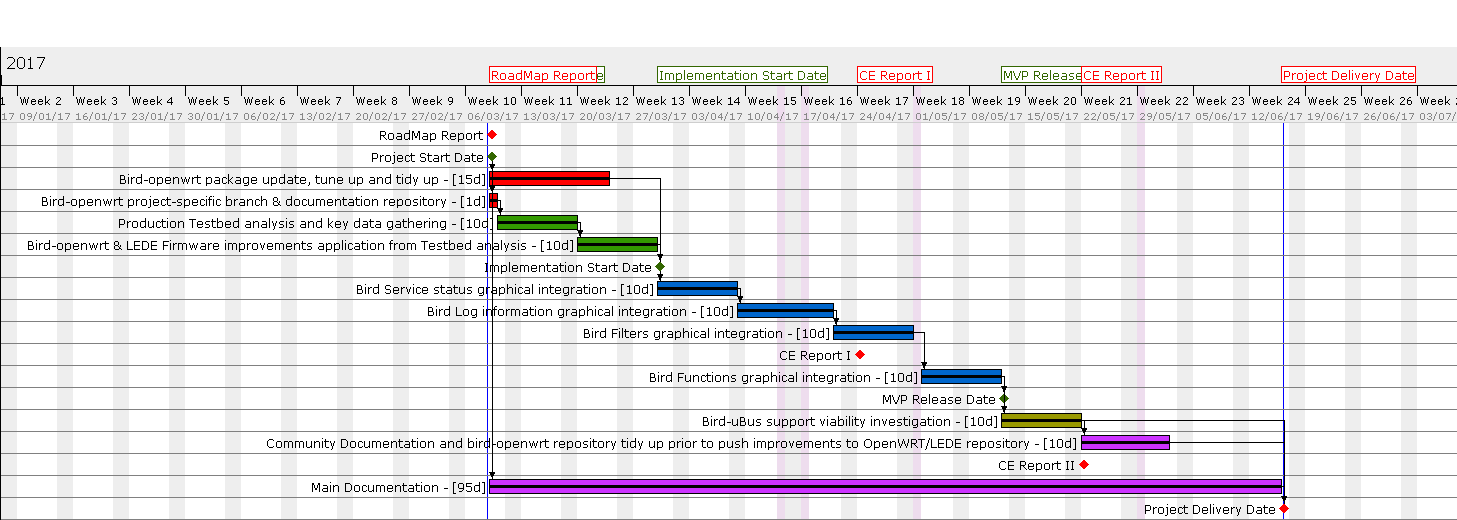
\includegraphics[width=\hsize]{images/gantt}
    \caption{Tasks schedule}
    \label{fig:general_gantt}
\end{figure}

Key milestones:
\begin{itemize}
    \item \textbf{Project's start date \& RoadMap Report} (09/03/17): initial Package refresh and production environment investigation. Project's goals formal report and when they are expected to be delivered.
    \item \textbf{Project's implementation start date} (30/03/17): beginning of features' implementation.
    \item \textbf{Continuous Evaluation Report I} (22/04/17): formal report to present Project's progress, pending work, any issue or blocker and updated  timeline.
    \item \textbf{MVP Release} (12/05/2017): forecast delivery date of the final version of the Package. No extra changes planned unless the investigation task requires them.
    \item \textbf{CE Report II} (22/05/17): optional progress report prior to Project's delivery.
    \item \textbf{Project Delivery Date} (12/06/17): final date to deliver the dissertation, slides, recording and any extra archive required.
\end{itemize} 

\begin{figure}[h!]
    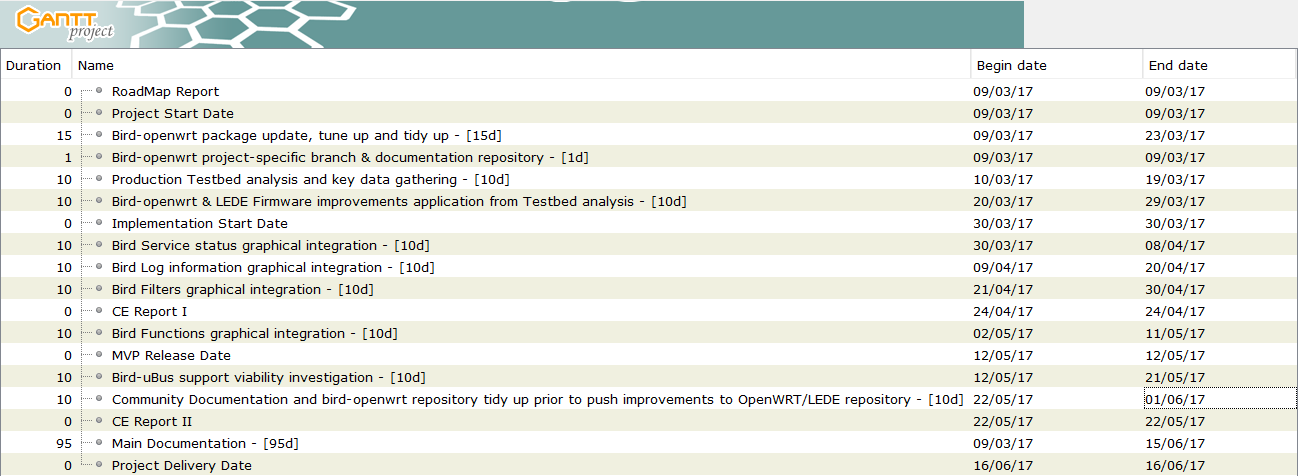
\includegraphics[width=\hsize]{images/gantt_data}
    \caption{Schedule details}
    \label{fig:detail_gantt}
\end{figure}
\end{landscape}


\section{Obtained results' brief summary}
This project has two main achievements:

The first one is the self-contained major update for bird-openwrt package, which has not only brought support for the latest Bird Daemon API, but also introduced a number of new functionalities and process automations critical for its adoption by our target administrators and the rest of OpenWrt's community.
The second main achievement is the detailed uBus integration analysis including some implementation examples and foreseen future development paths. As part of the analysis, I have also detailed a possible project proposal following the most promising implementation path for future students willing to learn about OpenWrt/LEDE, Bird Daemon and uBus communication architecture.

All contents mentioned in this dissertation are available on GitHub:

\begin{itemize}
    \item Bird-OpenWrt Package: \\
    \href{https://github.com/eloicaso/bird-openwrt}{https://github.com/eloicaso/bird-openwrt}
    \item Project's extra documentation:\\
    \href{https://github.com/eloicaso/bgp-bmx6-bird-docn}{https://github.com/eloicaso/bgp-bmx6-bird-docn}
    \item This dissertation:\\
    \href{https://github.com/eloicaso/msc_dissertation}{https://github.com/eloicaso/msc\_dissertation}
\end{itemize}

\section{Structure of the document}
\label{sec:sod}
This dissertation is organized as follows: Chapter \ref{ch:introduction} introduces background concepts to understand this project's scope and basic management information. Chapter \ref{ch:architecture} presents target and tested network architectures and its requirements. Chapter \ref{ch:implementation} goes in depth detail about which have been Package's main improvements and also briefly describing previous capabilities. Moreover, this chapter also details the theoretical analysis done on Bird's uBus integration feasibility. Chapter \ref{ch:tresults} brings exhaustive information regarding performed tests in both initial development and virtual real scenario networks, detailed information of the main differences between the original Package version and this project's enhancements, and also, common Bird errors and how to solve them. Finally, Chapter \ref{ch:conclusions} summarises main achievements, main challenges and whether they have been solved or not and also future development lines. 

